% This is the start of every LaTeX document. The document class specifes the overall type of
% document you are writing. 'article' is most common. 'report' is similar to 'article', but allows
% for chapters. 'book' is for writin large books. 'beamer' for making presentations
\documentclass{article}

% Below are all the included packages. Packages add extra functionality to default LaTeX by adding
% new macros or changing default behaviours
\usepackage[margin=35mm]{geometry} % Controls layout of the page, including margins
\usepackage[style=apa]{biblatex}              % Controls bibliography and citations
\usepackage{listings}              % Source code layout, formatting and styling
\usepackage{color}                 % Needed for coloring source code syntax
\usepackage[hidelinks]{hyperref}   % Support for links. Autolinks citations, references, and TOC
\usepackage{amsmath}               % Maths equations and aligns
\usepackage{amssymb}               % More maths symbols
\usepackage{graphicx}              % For including images
\usepackage{subcaption}            % For using subfigures
\usepackage{booktabs}              % For prettier looking tables and better rules

% Sets the title and author of the document. This is printed by \maketitle
% If date is not specified with \date{}, the current date is used
\title{\LaTeX{} Workshop}
\author{Tim Quelch}

% Add the references to the bibliography
\addbibresource{references.bib}

% Style options for souce code blocks (listing environment, and \lstinline{} macro)
\lstset{
	language=TeX,              % Language for syntax highlighting
	basicstyle=\ttfamily,      % Style for fonts
	numbers=left,              % Line numbers
	numberstyle=\tiny,         % Line number style
	frame=tb,                  % Frame lines on top and bottom
	tabsize=4,                 % Size of tabs
	columns=fixed,             % Fix character columns
	showstringspaces=false,    % Don't underscore spaces
	showtabs=false,            % Don't underscore tabs
	keepspaces,                % Keep spaces as spaces, not whitespace
	commentstyle=\color{red},  % Colour comments as red
	% keywordstyle=\color{blue},% Colour keywords as blue
	breaklines=true,           % Break lines, so they don't go over the page
}

% TODO config section numbers
% TODO config font selection
% TODO config fancy header

% All the actual content of the document goes in the document environment
\begin{document}

% Prints the title, author, and date.
\maketitle

% Prints the table of contents generated from the sections
\tableofcontents
\listoffigures
\listoftables

% Inserts a page break (new page)
\newpage

\section{Introduction}
``\LaTeX{} is a high-quality typesetting system; it includes features designed for the production of technical and scientific documentation. \LaTeX{} is the de facto standard for the communication and publication of scientific documents. \LaTeX{} is available as free software.''
\parencite{latex_project_latex_2018},

One of the key differences in \LaTeX{} to more common work processors (MS Word, LibreOffice etc.) is the separation of content and presentation. In \LaTeX{} the author describes the general structure of the document (section headings, paragraphs, equations, figures), and the layout and typesetting is handled by \LaTeX{} (or rather the underlying \TeX{} backend).

There are several advantages to this:
\begin{itemize}
  \item Author can focus on the actual content, rather than making everything look pretty
  \item Presentation can be changed easily without major formatting reworks throughout the document
  \item A standard(ish) format for submission to external publishers, who can then apply their own layout/presentation styles
\end{itemize}

\LaTeX{} is written in plain text, and is processed by an external program to generate the output files (usually a PDF)

\subsection{Pronounciation and Spelling}
\LaTeX{} is always \emph{lah-tech}, and sometimes \emph{lay-tech}. It is never pronounced \emph{lay-tecks}. It is always written with the \lstinline|\LaTeX{}| macro (output is the weird sized and spaced \LaTeX{}), or with the capitialistaion LaTeX.

\subsection{Language Structures}
There are two major language structures that you will encounter when using \LaTeX{}: macros, and environments.

Macros are how we tell \LaTeX{} to do things. They take the general form of \lstinline{\commandname}, or with arguments \lstinline|\commandname[optional args]{required args}|. Macros can do anything from printing the table of contents (\lstinline{\tableofcontents}), \emph{emphasising} or \textbf{bolding} text (\lstinline|\emph{emphasising},\textbf{bolding}|), or even printing the funny \LaTeX{} logo (\lstinline|\LaTeX{}|). It is even possible to define your own macros to simplify things you are repeating often.

Environments are how we write larger sections of the document which often contain many lines or macros. Environments begin with a \lstinline|\begin{environmentname}| macro, and end with a \lstinline|\end{environmenname}| macro. Common environments include \lstinline{figure}, \lstinline{equation}, \lstinline{itemize} (these will be discussed later).

\subsection{The Preamble}
The preamble contains all the configuration and setup before the actual content.

The first line of the preamble is setting the \lstinline{\documentclass}. This tells \LaTeX{} what kind of document you are writing. The most common one used is \lstinline{article}. Other ones include \lstinline{report} which is similar to \lstinline{article}, but allows for chapters. \lstinline{book} is for writin large books. You can even write powerpoint presentations with the \lstinline{beamer} class.

The preamble also includes all the package inclusions for the document with the \lstinline|\usepackage{packagename}| macro. Packages add extra functionality to default \LaTeX{} by adding new macros or changing default behaviours. For example, the \lstinline{amsmath} package adds support for more maths environments and symbols, \lstinline{graphicx} allows for the inclusion of image files for figures.

Any extra configuration for styling and layout is also done in the preamble.

\subsection{\lstinline{document} Environment}
All of the actual content of the document goes in the \lstinline{document} environment.

\section{Useful structure things} % TODO rename?

\subsection{Sections}
Sections are used to divide the document into parts. A new section is started with the \lstinline|\section{sectionname}| macro. Section titles are formatted to be bigger, bolded, and automatically numbered.

The table of contents (\lstinline{\tableofcontents}) is generated from the section headings. All the page numbers and section numbers are set automatically.

\subsection{Subsections}
We can also split sections into smaller \lstinline|\subsection{subsectionname}|
\subsubsection{Subsubsection}
... and \lstinline|\subsubsection{subsubsectionname}|

\subsection*{Unnumbered sections}
Sections and subsections can be unnumbered if they are declared with an asterisk. e.g.\ \lstinline|\section*{section name}|. The current subsection is un numbered in this way

\subsection{Lists}
\label{sec:lists}
Dot point lists are created with the \lstinline{itemize} environment
\begin{itemize}
  \item Each item begins with the \lstinline{\item} macro
  \item another item
    \begin{itemize}
      \item You can also do nested lists by just starting a new \lstinline{itemize} environment
        \begin{itemize}
          \item And the marker changes for each level you are on
            \begin{itemize}
              \item List markers and spacing and spacing can be customised with the \lstinline{enumitem} package
            \end{itemize}
        \end{itemize}
    \end{itemize}
\end{itemize}


Numbered lists are created with the \lstinline{enumerate} environment
\begin{enumerate}
  \item Each item begins with the \lstinline{\item} macro
  \item another item
    \begin{enumerate}
      \item You can also do nested lists by just starting a new \lstinline{enumerate} environment
        \begin{enumerate}
          \item And the marker changes for each level you are on
            \begin{enumerate}
              \item List markers and spacing and spacing can be customised with the \lstinline{enumitem} package
            \end{enumerate}
        \end{enumerate}
    \end{enumerate}
\end{enumerate}

\section{Maths}

One of \LaTeX{}'s strengths is the formatting of maths. The easiest way to layout maths is with the inline maths mode, which is used by surrounding expressions with \$s. e.g.\ $a + b = c$. \LaTeX{} automatically handles spacing and formatting of maths.

In order to print an equation on its own line, you can use the \lstinline{equation} environment. To make things super script, \lstinline{^} is used, and to make things subscript, \lstinline{_} is used. Fractions are formatted with the \lstinline|\frac{numerator}{denominator}| macro
\begin{equation}
    a^2 + b^2  = \frac{r}{c}
\end{equation}

The \lstinline{equation} environment only allows for a single line of maths, if multiple lines are required, the \lstinline{align} environment can be used. In addition to allowing multiple lines, \lstinline{align} also allows you to align each line at a point specified by an \lstinline{&}. Below, each line is aligned on the $=$ sign.

\begin{align}
  0 &= ax^2 + bx + c \\
  0 &= a(x^2 + \frac{b}{a}x) + c \\
  a \left( \frac{b}{2a} \right)^2 &= a \left( x^2 + \frac{b}{a}x + \left( \frac{b}{2a} \right)^2 \right) + c \\
  \frac{b^2-4ac}{4a^2} &= \left( x +\frac{b}{2a} \right)^2 \\
  x &= \frac{-b \pm \sqrt{b^2 - 4ac}}{2a}
\end{align}

If you want to write normal text in maths mode, you need to use the \lstinline{\text} macro

\begin{align}
  \text{this text is written in text mode} \\
  this text is written in math mode
\end{align}

\LaTeX{} provides a lot of different  symbols that can be  used in math mode including the greek alphabet (shown below). A more extensive list can be found at \href{https://www.rpi.edu/dept/arc/training/latex/LaTeX_symbols.pdf}{The Great, Big List of \LaTeX{} Symbols} \parencite{carlisle_great_2001}

\begin{equation}
    \alpha \beta \gamma \delta \epsilon \varepsilon \zeta \eta \theta \vartheta \iota \kappa \lambda \mu \nu \xi \pi \varpi \rho \varrho \sigma \varsigma \tau \upsilon \phi \varphi \chi \psi \omega
\end{equation}
\begin{equation}
    \Gamma \Delta \Theta \Lambda \Xi \Pi \Sigma \Upsilon \Phi \Psi \Omega
\end{equation}

Bringing all of these together can give pretty equations like:
\begin{equation*}
    v = \frac{2}{L} \sum_{n=1}^\infty e^{-(\kappa \beta_n^2 + \nu) t} \cos{(\beta_nx)}
    \left(
        \kappa \beta_n(-1)^n
        \int_0^t e^{(\kappa \beta_n^2 + \nu)\lambda}\phi(\lambda) d\lambda +
        \int_0^L f(x') \cos{(\beta_nx')} dx'
    \right)
\end{equation*}
\begin{equation*}
    v = T - T_f, \quad \kappa = \frac{k}{\rho c}, \quad \nu = \frac{h p}{\rho c A}, \quad \beta_n = \frac{\pi}{2L}(2n + 1)
\end{equation*}

\newpage
\section{Figures, Tables, and Code}

Figures and tables can be added to the document either raw or by using floats. Floats let \LaTeX{} algorithmically place the figures in the document to look good. The float environment for figures is \lstinline{figure} and for tables is \lstinline{table} (suprise suprise). Floats are containers for objects which can't be displayed over multiple pages. Floats should always have a caption to describe them (with \lstinline{\caption}), as they do not always appear where they appear in the source code.

\begin{figure}[h]
    \centering
    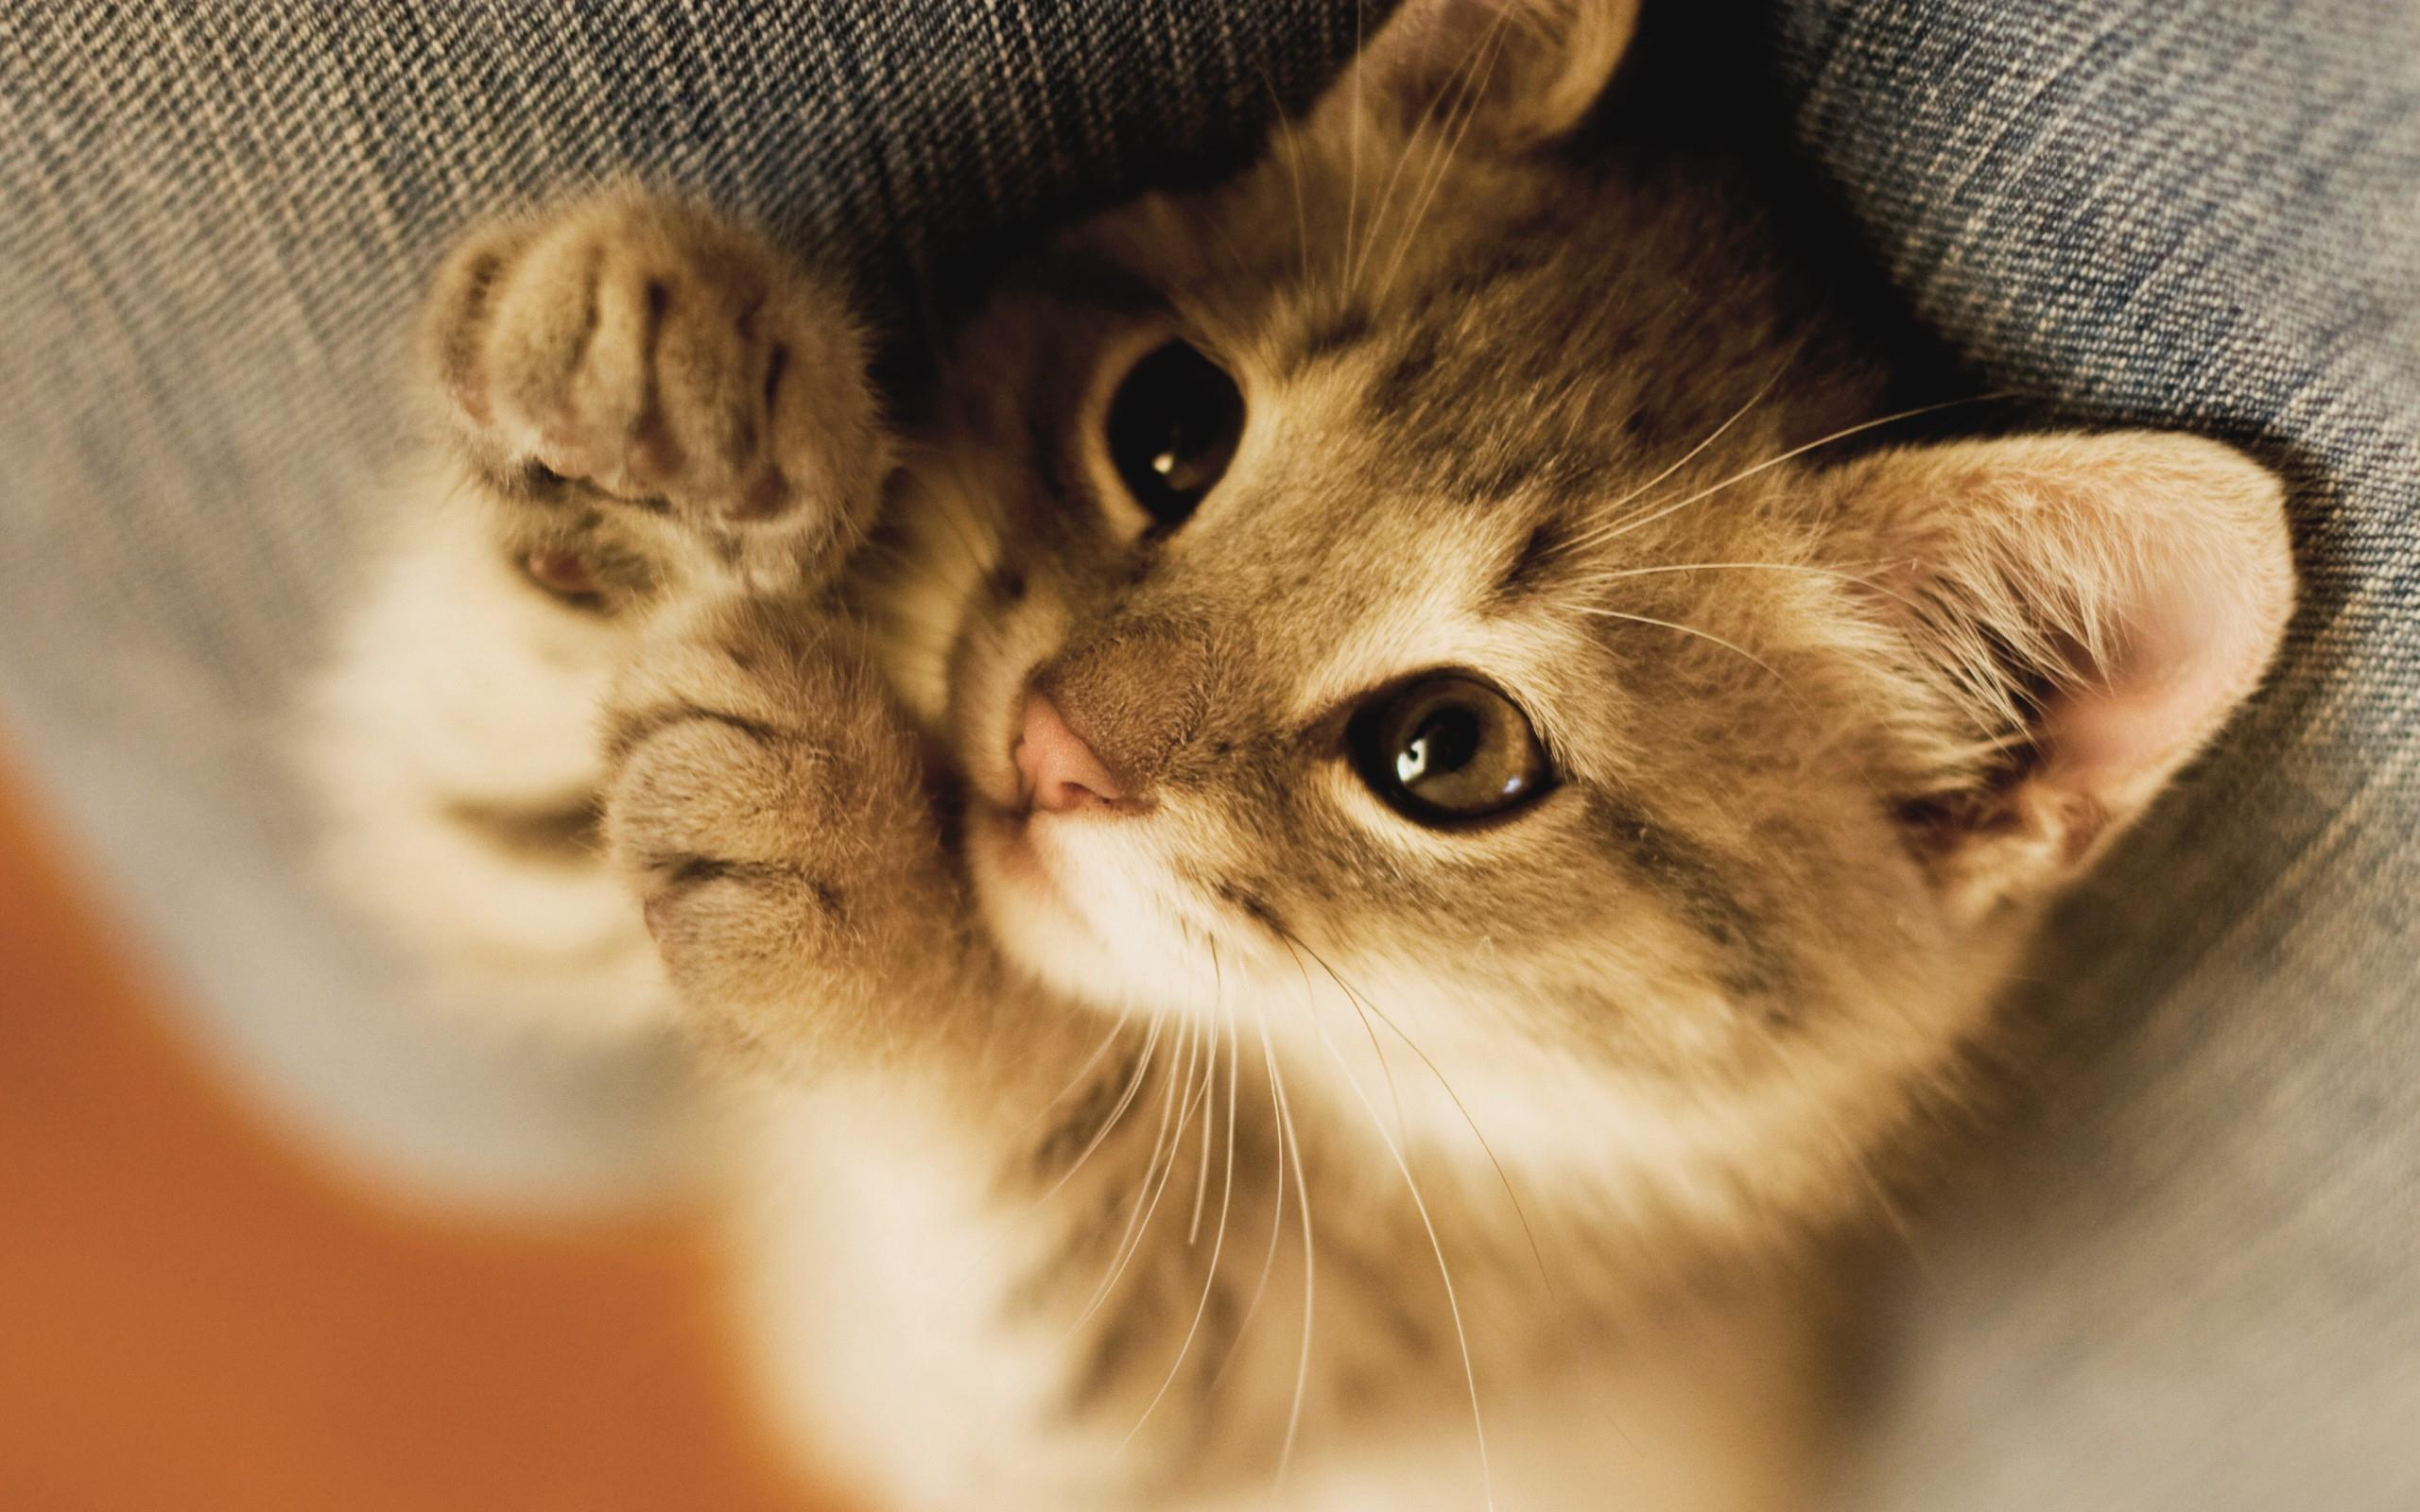
\includegraphics[width=0.7\textwidth]{cat.jpg}
    \caption{This is a caption for the figure. The figure numbering is automatic}
    \label{fig:cat}
\end{figure}

\begin{figure}[h]
    \centering
    \begin{subfigure}{0.47\textwidth}
        
\includegraphics[height=5.5cm]{rabbit.jpg}
        \caption{The first subfigure}
    \end{subfigure}
    ~
    \begin{subfigure}{0.47\textwidth}
        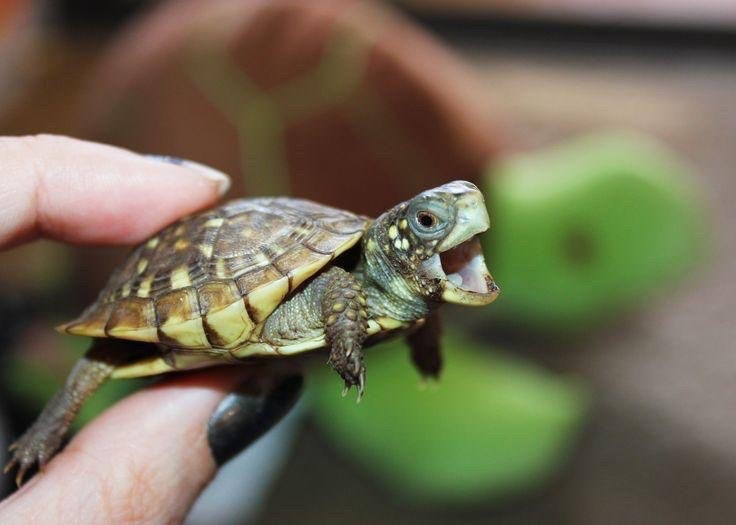
\includegraphics[height=5.5cm]{turtle.jpg}
        \caption{The second subfigure}
        \label{fig:turtle}
    \end{subfigure}
    \caption{A caption for both subfigures}
\end{figure}

\begin{table}[h]
    \centering
    \caption{An example table. This generally goes above the table}
    \begin{tabular}{lrr}
      \toprule
      & Column 1 & Column 2 \\
      \midrule
      Row 1 & 7 & 2 \\
      Row 2 & 8 & 9 \\
      Row 3 & 2 & 0 \\
      Row 4 & 4 & 1 \\
      \bottomrule
    \end{tabular}
\end{table}

Lists of figures and tables can be printed similarly to a table of contents with \lstinline{\listoffigures} and  \lstinline{\listoftables}

Source code can also be included with the \lstinline{listing} environment. In addition to the environment, code can also be included with the \lstinline{\lstinline} macro (this is what I have been doing for all the macros in this document)

\begin{figure}
\caption{An example listing}
\begin{lstlisting}[language=c++,keywordstyle=\color{blue}]
#include <iostream>

int main() {
    std::cout << "Hello World!" << std::endl;
    return 0;
}
\end{lstlisting}
\end{figure}

\subsection{References \& Labels}
Throughout this document you may have noticed that everything is numbered (e.g. equations, sections, figures, tables). It is incredibly easy to refer to these things with the label and reference system in \LaTeX{}. Everything that is numbered (and some things that are not) can have a label attached with the \lstinline|\label{labelname}| macro. The number can then be later refered to with the \lstinline|\ref{labelname}| macro. This means that if you go back and add a figure, all your reference to later figures will be automatically updated to reflect the new figure names.

Even better, when the \lstinline{hyperref} package is included (by \lstinline|\usepackage{hyperref}| in the preamble), all of these references are turned into hyperlinks to the item. This means that you can click on a reference and go straight to the related equation, figure, or table. This package also turns all the entries in the table of contents and table of figures into a link, to allow for easy navigation of the document

If you want to reference the page that a label is on, you can do that with the \lstinline|\pageref{labelname}| macro.
Below are some examples of references.
\begin{itemize}
  \item Reference to a figure -- Figure \ref{fig:cat}
  \item Reference to a subfigure -- Figure \ref{fig:turtle}
  \item Reference to table -- Table \ref{tab:placement-specs}
  \item Reference to a section (with pageref) -- Section \ref{sec:lists} on page \pageref{sec:lists}
\end{itemize}

\subsection{\LaTeX{} (usually) knows better than you}
A mistake many people new to \LaTeX{} make is trying to force images to go in particular places. This is often very hard and not necessary. \LaTeX{} is very good at placing floats in places that look good, and do not break the flow or layout of the document too much.

There are several placement specifiers that we can provide to the float commands in order to give \LaTeX{} hints on where we want the float to go. These go right after begin float macro. e.g. \lstinline|\begin{figure}[placement specifier] ... \end{figure}|. Table~\ref{tab:placement-specs} shows all of the available placement specifiers.

\begin{table}
    \centering
    \caption{Placement specifiers for floats. Multiple of these can be specified}
    \label{tab:placement-specs}
    \begin{tabular}{ll}
      \toprule
      Spec. & Location \\
      \midrule
      h & Place \emph{approximately} here \\
      t & Place at top of page \\
      b & Place at bottom of page \\
      p & Place on page for only floats \\
      ! & Override internal placement parameters (force placement) \\
      \bottomrule
    \end{tabular}
\end{table}

% TODO

\section{Citations}
There are many ways to manage bibliographies, citations, and reference lists in \LaTeX{}, and many of them are outdated or have been superseded by newer alternatives. The method that I use is with a combination of BibLaTeX and Biber. BibLaTeX is the frontend in \LaTeX{} that handles citations and printing the bibliography. Biber is the backend which manages the database of all the references.

References are stored in a database file with a \lstinline{.bib} extension. An example database file for the sources used in this document is shown below (note: I am including the file with \lstinline|\lstinputlisting{filename}|, which turns a file into a source code listing). Each entry in the database file refers to an source, with the necessary fields filled. 

These sources can be cited with \lstinline|\cite{referencename}| (no parentheses) or \lstinline|\parencite{referencename}| (with parentheses). For example \parencite{strzodka_gpu-accelerated_2013} \parencite{yu_gpu_2014}

\lstinputlisting{references.bib}



\printbibliography

\end{document}